%% simulationSoftware.tex
%%

%% ==============
\chapter{Simulation of Background Inducing Muons}
\label{ch:Simulation of muon induced background}
%% ==============
  To compare the data aquired to theoretically expected values, a Geant4 \cite{geant} simulation of cosmic showers has been set up including the geometry of the main spectrometer as well as the muon modules. Using this software, inciding muons can be simulated and the effect on the main spectrometer and the muon modules can be evaluated. It was especially relevant to achieve estimations on how many of the main spectrometer penatrating muons are registered by the muon modules. From this simulation, the overall rate of muon impacts on the main spectrometer can be obtained. Comparing this overall rate to detector rates for asymmetric fields can give clues on the probability of a muon hitting the main spectrometer inducing an electron.
  %% ===========================
  \section{Geant4}
  \label{ch:Simulation software:sec:Geant4}
  %% ===========================
  The Geant4 package is a powerful tool for simulation of particles. It has many particle interactions already included making it easy for the user to set up and run simulations. To start a run, geometry, one ore multiple detectors and interactions have to be defined. Each run may consist of one or more events. During a single run, a loop of processes is called:
  \begin{enumerate}
  	\item Primary Generator Action
  	\item Run action
  	\item Event action
  	\item Stacking action
  	\item Tracking action
  	\item Stepping action
  \end{enumerate}
  Each run usually contains many event actions and every event action multiple tracking actions. For each item above, classes with the addition 'user' to the base classes name can be called before or after the standard action class. These are used to extract the required data. In this simulation for every event in which a muon module has been hit, its copy number is pushed back to a vector of event data. The visualization of the simulated data is controlled via ``.mac'' file, by default the ``vis.mac'' file. Different parameters can be changed and simple visualisation settings like viewing angles and zooms can be chosen. An example is given in annex \ref{ch:annex:sec:vis.mac}.
  


  %% ===========================
  \section{Geometry Setup}
  \label{ch:Simulation software:sec:Geometry setup}
  %% ===========================
  To set up a geometry, the class G4VUserDetectorConstruction is used. B1DetectorConstruction inherits from that as a base class and additionally contains all of the geometrical parameters needed for the setup such as radii of the main spectrometer cones or positions and extent of the muon modules. Every shape generated is made up of both a logical volume G4LogicalVolume and a physical volume G4PhysicalVolume. The logical volume describes the intrinsic properties of the geometric object added: its shape, its size and its material. The physical volume accepts a logical volume as input providing position and alignment of the previously defined.
  Inside the detector construction class, all of the materials used in the simulation need to be defined as well. These are the components of the air outside and inside the spectrometer including pressures and constitution, the stainless steel of the spectrometer wall and the scintillator material of the muon modules.
  The main spectrometer geometry was already existant (see \cite{mainSpecGeometry}) but had to be modified as many border volumes were implemented. These were very flat volumes covering any area of the main spectrometer not needed for this simulation. Additionally, the muon modules were added as sensitive volume. Keeping in mind that one wants to not only distinguish whether a module has been hit, but also which one. That is why the logical volume for every module is the same whereas the physical volume is a copy of the first at different world coordinates making them identifiable via their individual copy number. A screenshot of the visualized geometry setup including a hit of one of the modules is shown in \ref{fig:geant:geometry}.
  
  \begin{figure}
  	\centering
  	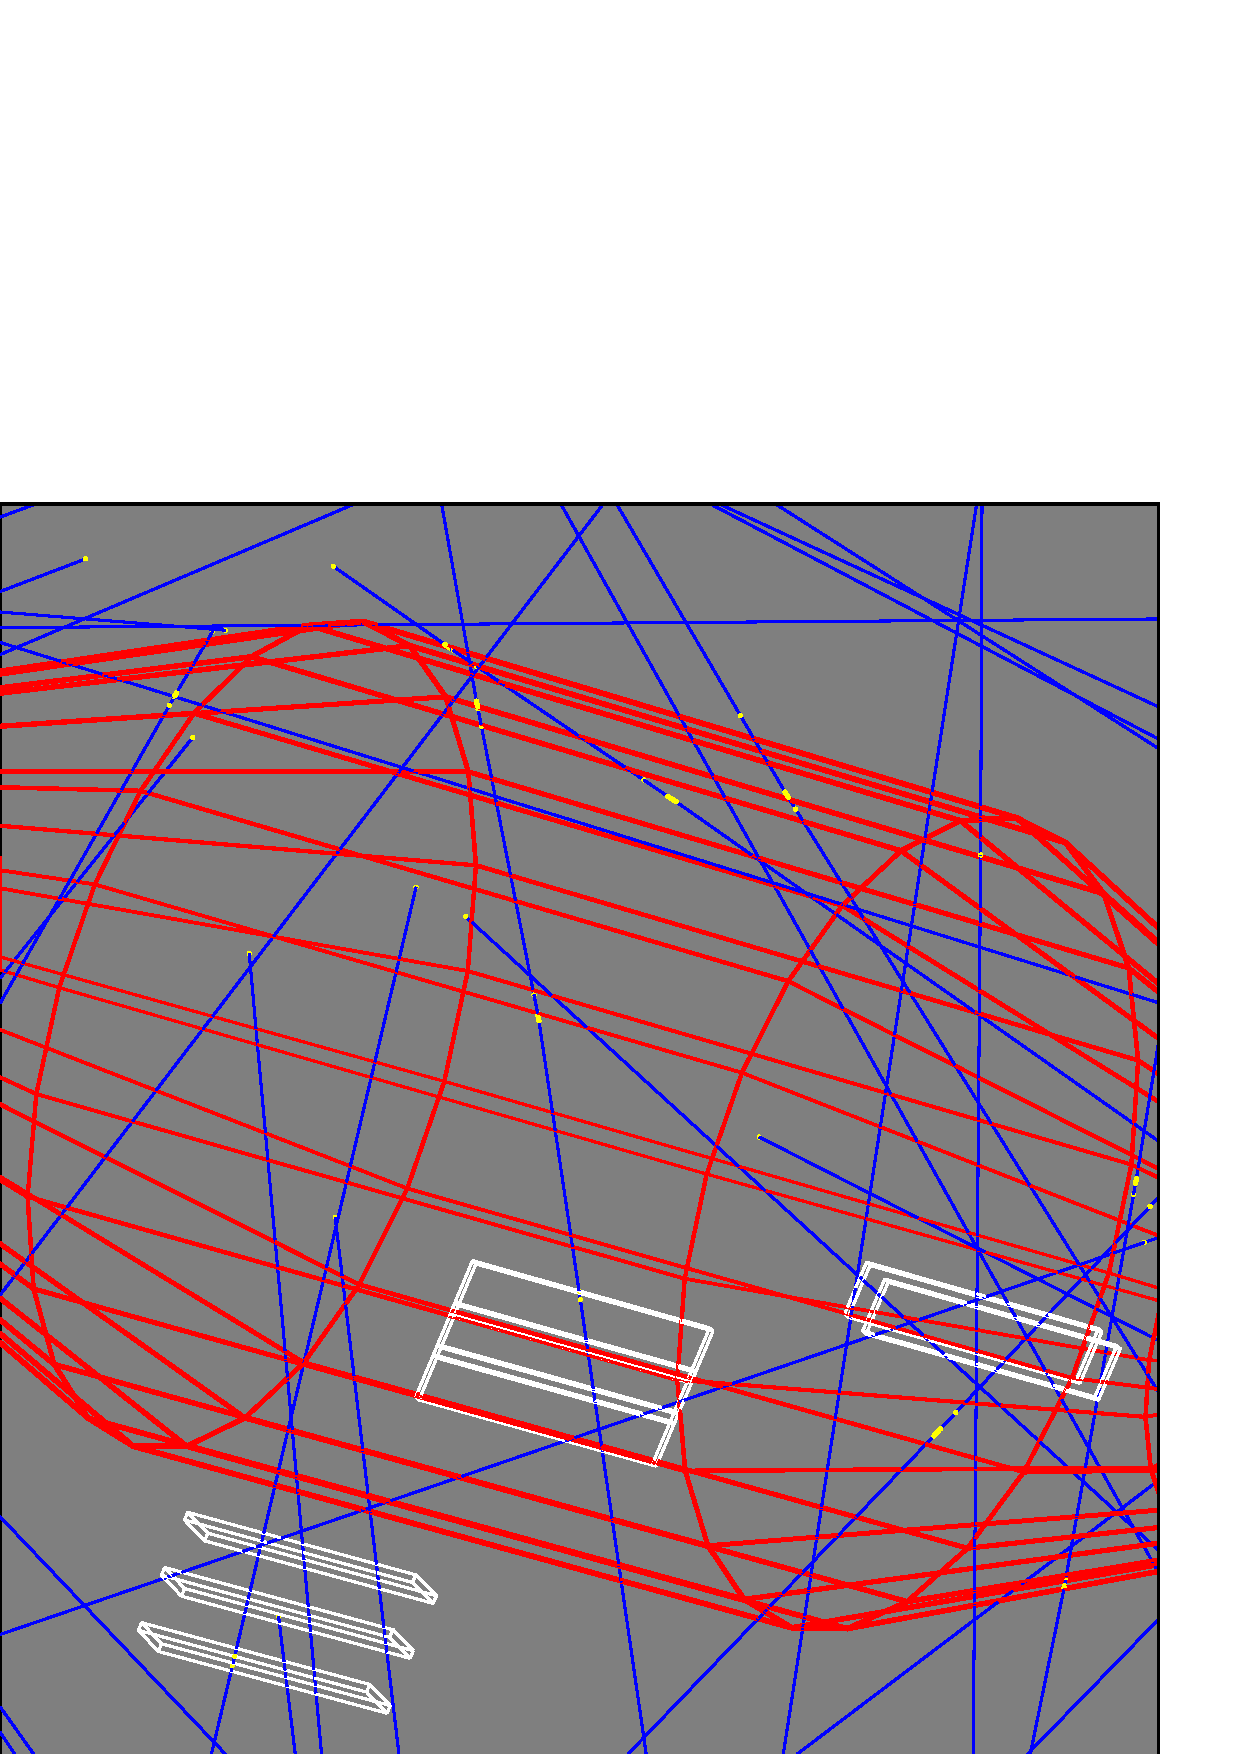
\includegraphics[width = 0.5\textwidth]{graphics/simulation/moduleHit.png}
  	\caption[Simulation geometry setup]{Screenshot of the geometry setup and muon paths in the OpenGL viewer. The view is upwards through the main spectrometer standing on the west side of it. The three groups of muon modules (white) are visible right below the large main spectrometer structure (red). A variety of incident muons is shown (blue). Hits are marked (yellow) by the Geant4 viewer. A single muon's hits are marked with black circles. Both entry and exit point into and out of the main spectrometer and the detection point are visible.}
  	\label{fig:geant:geometry}
  \end{figure}

  
  %% ===========================
  \section{Muon Generator}
  \label{ch:Simulation software:sec:Muon generator}
  %% ===========================  
  
  The muon generation was realized through the primary generator action. The angular distribution suggested by Henrik Arlinghaus \cite{DTArlinghaus} was implemented. The angular rate dependence is shown in \ref{fig:rateDependance}. The energy was set to \todo{reasonable value} disregarding the actual energy distribution as this was mainly about flight paths that are not strongly dependent on energy at high energies. Starting positions were spherically distributed, with the direction towards the origin, which is in the center of the main spectrometer. Starting positions were then randomly moved in a volume surrounding the spectrometer to account for the non-point like structure of the detection system as a whole, while the distribution describes a single point in space.
  \begin{figure}
  \centering
  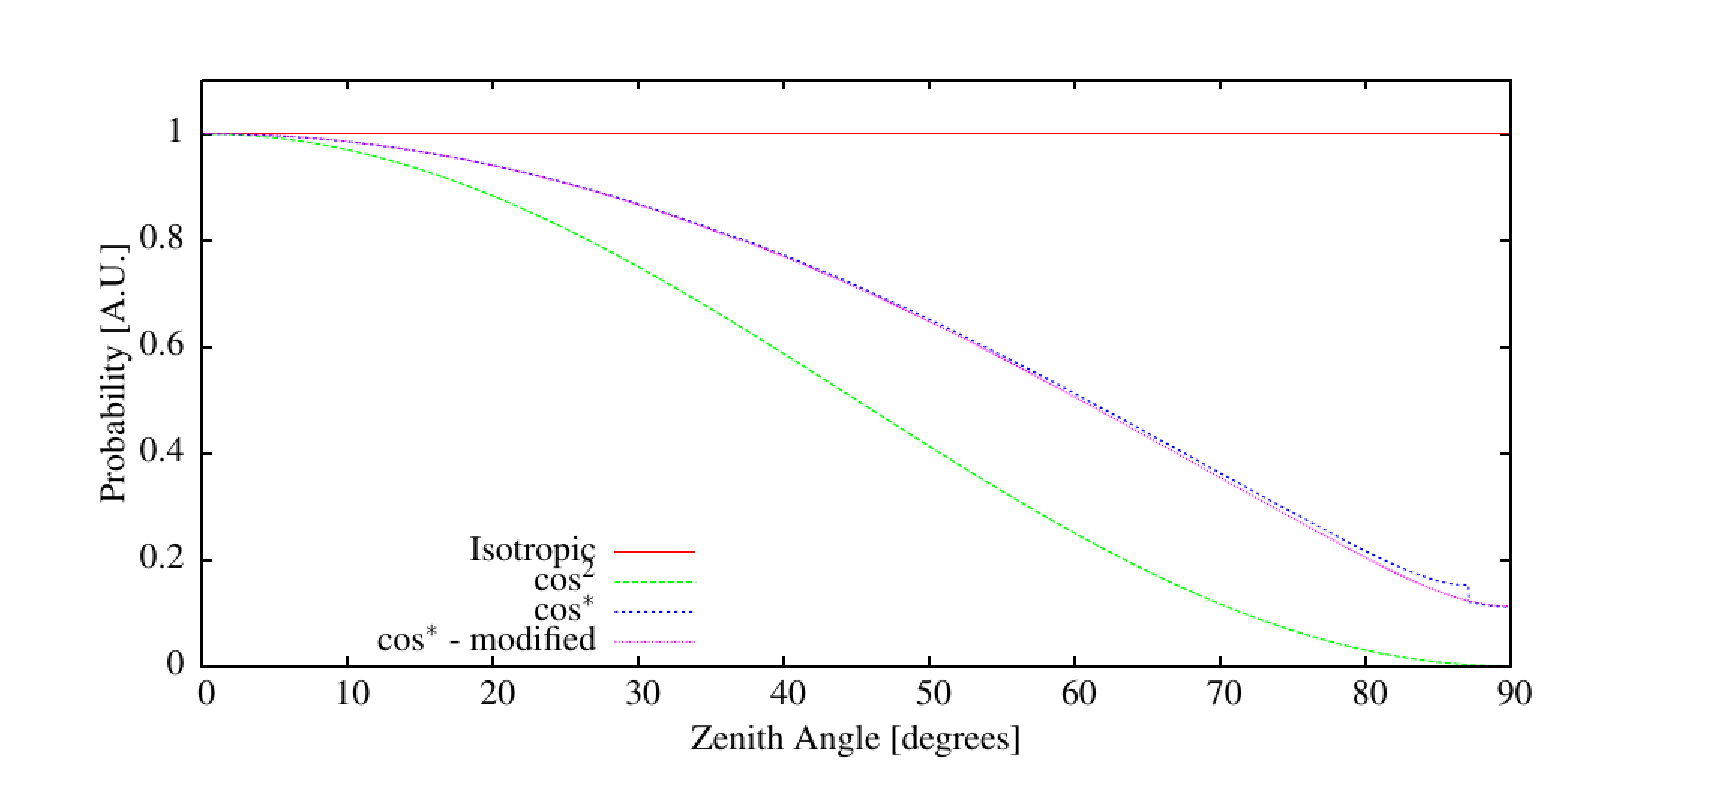
\includegraphics[width = 0.8\textwidth]{graphics/simulation/angularDistributions.eps}
  	\caption[Muon rate dependance on zenith angle]{Different angular distributions. Isotropic and $\cos^2$ distributions are shown opposed to the $\cos^*$ distribution. The latter is plotted with and without a wrongly published parameter from the original publication \cite{distro}.}
  	\label{fig:rateDependance}
  \end{figure}
  The distribution used is the cos* distribution.
  \begin{equation}
  	\cos^*{\left(\theta \right)} = S(\Theta)\cos^{**}{\left(\theta\right)}
  \end{equation}
  with
  \begin{equation}
  	S(\theta) = 0.986 + 0.0007\sec{\theta}
  \end{equation}
  and $S(\theta)$ described by a polynomial
  \begin{equation}
  	\cos^{**} = \sum_{i=0}^{4}{c_i \cos^i{\theta}}.
  	\label{eq:coeffs}
  \end{equation}
  The coefficients are defined differently for different angular ranges shown in table \ref{tab:coefficients}.
  \begin{table}
  \centering
  	\begin{tabular}{|c|c|c|c|c|c|c|}
  	\hline
  		$\cos{\left(\theta\right)}$ & $c_0$ & $c_1$ & $c_2$ & $c_3$ & $c_4$ & max. rel. error\\
  		\hline
  		0 - 0.002 & 0.11137 & 0 & 0 & 0 & 0 & 0.004\\
	
  		0.002 - 0.2 & 0.11148 & -0.03427 & 5.2053 & -14.1971 & 6.138 & 0.3\\
  		0.2 - 0.8 & 0.06714 & 0.71578 & 0.42377 & -0.19634 & -0.021145 & 0.7\\
  		\hline
  	\end{tabular}
	\caption[Angular distribution coefficients]{These are the coefficients for equation \ref{eq:coeffs}. Every set of coefficients is applicable to a certain angular region indicated in the first column. The last column shows the largest occurring relative error in each region. }
  \end{table}

  
  %% ===========================
  \section{Hit Counter}
  \label{ch:Simulation software:sec:Hit counter}
  %% ===========================
  
  To compare moun measurements and simulations, events with at least one module hit were counted.  This made it possible to compare the rates of the single modules, showing that the generator works fine. furthermore, it allowed for a estimation of muons hitting the modules compared to the total of inciding muons. Table \ref{tab:simResults} shows the result of a simulation generating \SI{e 6}{} particles and compares it to measured data. Of the particles generated, the single modules were hit \SI{506\pm 44}{} times. In the same period, the main spectrometer was hit almost \SI{6e4}{} times. This shows formidably that the detection system is by no means a veto system to discriminate muon induced events, but merely for background studies. To compare simulation to real data, a time scale had to be introduced. The nuber of events for a single module corresponds very well to \SI{2}{\second} of measurement time. Consequently, the simulation has been compared to the \SI{2}{\second} average of a half hour run. 
  \begin{table}
  \centering
  	\begin{tabularx}{0.7\textwidth}{|c|>{\centering\arraybackslash}X>{\centering\arraybackslash}X>{\centering\arraybackslash}X>{\centering\arraybackslash}X|}
  	\hline
  	module & 1 & 2 & 3 & 4\\
  	\hline
  	simulation & 550 & 534 & 499 & 410  \\
  	real data & 495$\pm$ 23 & 544 $\pm$ 24 & 497 $\pm$23 & 483$\pm$22 \\
	\end{tabularx}
	\begin{tabularx}{0.7\textwidth}{|c|>{\centering\arraybackslash}X>{\centering\arraybackslash}X>{\centering\arraybackslash}X>{\centering\arraybackslash}X|}
  	\hline
  	module  & 5 & 6 & 7 & 8 \\
  	\hline
  	simulation & 508 & 543 & 506 & 496 \\
  	real data & 490$\pm$23 & 498$\pm$23 & 510$\pm$ 23& 532$\pm$ 24 \\
  	\hline
  	\hline
	\end{tabularx}
  	\begin{tabularx}{0.7\textwidth}{|c|>{\centering\arraybackslash}X>{\centering\arraybackslash}X>{\centering\arraybackslash}X>{\centering\arraybackslash}X>{\centering\arraybackslash}X|}
  	modules & 1+2 & 6+7 & 7+8 & 6+7 & 6+7+8 \\
  	\hline
  	simulation & 204 & 135 & 130 & 66 & 66 \\
  	real data  & 191$\pm$14 & 136$\pm$12 & 146$\pm$12 & 65$\pm$8 & 62$\pm$8 \\
  	\hline
  	\end{tabularx}
  	\caption[Simulation comparison]{Comparison of the simulation data to ral data. }
	\label{tab:simResults}
  \end{table}
  Especially important is that the ratio of multi-module events to single module events is comparable. This can be used as a direct validation of the simulation's angular distribution. The different distances between the single modules are responsible for the difference in counts for multi-module events.
  The ratios are shown in table \ref{tab:}
  \begin{table}
  \centering
  \begin{tabular}{|l|c|c|c|c|c|}
  
  \hline
  	\rule{0pt}{4ex} ratio &$N_{12}/\bar N_{single} $&$ N_{67}/\bar N_{single}$ & $N_{78}/\bar N_{single} $& $N_{68}/\bar N_{single} $& $N_{678}/\bar N_{single}$\\
  	\hline
	simulation & 0.40 & 0.13 & 0.27 & 0.13 & 0.26\\
	real data & 0.38 & 0.27 & 0.29 & 0.13 & 0.12 \\
	\hline
  	\end{tabular}
  	\caption[Single \& Multi side event ratio]{The ration of a multi-module event is compared to the average rate of the single modules. Simulation and real data show comparable values.}
  \end{table}

  The simulation data can be used to estimate the probability of a muon inducing an electron at the detector after taking long term measurements with high statistics.
  Furthermore, by saving entry and exit points to ant out of the main spectrometer, a heatmap of the main spectrometer can be made. Particle tracking from these points with the already avaliable Kassiopeia software will provide more information on and improve the understanding of the background process.
  
  
  
  
  